\documentclass[11pt,psfig]{article}
\usepackage{epsfig}
\usepackage{times}
\usepackage{amssymb}
\usepackage{float}

\newcount\refno\refno=1
\def\ref{\the\refno \global\advance\refno by 1}
\def\ux{\underline{x}}
\def\uw{\underline{w}}
\def\bw{\underline{w}}
\def\ut{\underline{\theta}}
\def\umu{\underline{\mu}} 
\def\bmu{\underline{\mu}} 
\def\be{p_e^*}
\newcount\eqnumber\eqnumber=1
\def\eq{\the \eqnumber \global\advance\eqnumber by 1}
\def\eqs{\eq}
\def\eqn{\eqno(\eq)}

 \pagestyle{empty}
\def\baselinestretch{1.1}
\topmargin1in \headsep0.3in
\topmargin0in \oddsidemargin0in \textwidth6.5in \textheight8.5in
\begin{document}
\setlength{\parskip}{1.2ex plus0.3ex minus 0.3ex}


\thispagestyle{empty} \pagestyle{myheadings} \markright{G}



\title{CS 266 Homework 3}
\author{Zachary DeStefano, PhD Student, 15247592}
\date{Due Date: April 24, 2014}

\maketitle

\vfill\eject

\section*{Problem 3.11}

For this problem, it could end up not being monotone because of a concave vertex in the polygon that would cause there to be more than two intersection points in a given direction. We will thus go through each of the concave vertices and determine which directions that the polygon is not monotone in given that vertex. This will give us an interval of angles. Once we get the union of the intervals, we will see if that covers $[0,\pi]$ and if not, then the polygon is monotone for some direction. \\
\\
Here is the algorithm:\\
1. Initialize R to be empty. \\
2. For each vertex that is concave:\\
- Call the line segments through them $l$ and $l'$ \\
- Draw the lines perpendicular to $l$ and $l'$ and call them $L$ and $L'$\\
- Find the angles of $L$ and $L'$ with the x-axis and call them $\theta$ and $\theta'$. \\
- Find the min and max of $\theta$ and $\theta'$ and call them $\theta_1$ and $\theta_2$. \\
- Add $[\theta_1,\theta_2]$ to R.\\
3. Take the union of all the intervals in R. \\
4. If $[0,\pi] \subseteq R$, then the polygon is not monotone. \\
Otherwise it is monotone. 

\begin{figure}[H]
\centering
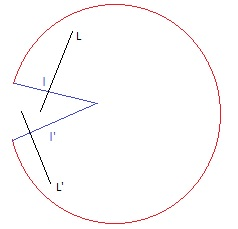
\includegraphics[height=3in]{monotone_diagram.jpg}
\caption{The non monotone directions with a concavity}
\end{figure}

Running time:\\
For each vertex, we do a constant number of operations. \\
Thus we have a total running time of $O(n)$

\newpage

\section*{Problem 3.14}

For this algorithm, we will go through each line segment in order and add the triangle it makes with $P$ to the visible region. If as we traverse the polygon we end up not going in clockwise order, then we will delete edges from the triangulation until we only have the visible ones. \\
\\
Here is the algorithm:\\
1. Initialize list L of current edges. \\
2. Initialize list T of triangles that make up visible region. \\
3. Start at the left most point on the polygon and add the next segment in clockwise order to L. \\
4. Add that first triangle to T. \\
5. Initialize $v$ to be the endpoint of the first segment. \\
6. For each segment $l$ in lexicographic order of the polygon:\\
If its endpoint $v'$ is after $v$ in clockwise order, then add $l$ to $L$ and add the triangle to $T$. \\
Otherwise, do the following: \\
- delete segments from the bottom of $L$ until one of them, $l'$, intersects the line formed by $P$ and $v'$. Call the point $p'$. \\
- delete the corresponding triangles from $T$. \\
- delete the triangle formed by $l'$ and add in the one formed by $P$, $p'$ and the visible endpoint of $l'$. \\
Once you are done processing this segment, set $v$ to be its endpoint. \\
7. The set of triangles $T$ forms the visible region. \\
\\

\begin{figure}[H]
\centering
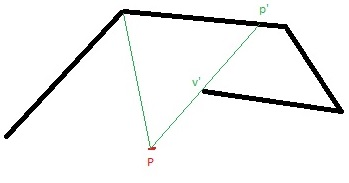
\includegraphics[height=3in]{reordering_case.jpg}
\caption{Diagram of a case where you need to redo the visible region}
\end{figure}

Running time:\\
There are $n$ iterations of the loop and each has a constant number of operations unless a reordering needs to be done. \\
Segments will not be deleted more than once so the total number of times something is deleted will not be more than n. \\
The total running time is thus $O(n)$. 



\newpage

\section*{Problem 15.2}

If we take two points $a$ and $b$ and get their duals, $a*$ and $b*$, these lines will intersect assuming that $a$ and $b$ have different x-coordinates. \\
Denote their intersection point as $p*$\\
The dual of $p*$, which is the line $p$ in the primal plane will go through $a$ and $b$. \\
Thus, the x-coordinate of $p*$ tells us the slope of the line through $a$ and $b$. \\
\\
There is a direct relationship between slope and angle. \\
In the right half-plane the slope increases in counter-clockwise order from $-\infty$ to $\infty$. \\
In the left half-plane, the slope increases in clockwise order from $-\infty$ to $\infty$. \\
This means that if we split up the points into left and right half and then order them by the slopes, we will be able to get the radial order of the points. \\
\\
We can now translate these facts into a new algorithm:\\
1. Dualize the points\\
2. Compute the arrangement of the duals. \\
3. For each vertex v in the primal plane:\\
- Find the line v* in the dual and get its intersection points in the dual in x-coordinate order. \\
- Go through the points and put the ones corresponding to the left points into $points_{left}$ and right points into $points_{right}$. \\
- concatenate $points_{left}$ in increasing order with $points_{right}$ in decreasing order to get vertices in radial order. \\
\\
Running time:\\
Computing the arrangement takes O($n^2$). \\
Since the arrangement was computed, there is no need to sort when finding the intersection points for $v*$ thus that step is O(n). \\
This means that step 3 take O($n^2$). \\
The total running time is thus O($n^2$) which is an improvement over the last algorithm. 


\newpage

\section*{Problem 15.4}

We can construct an instance where we have $2^{n/2}$ shortest paths, giving us a lower bound on the maximal number of shortest paths. \\
1. Put equal sized triangles between two points $s$ and $t$. \\
2. Between those triangles put very large triangles. \\
3. This will cause the shortest paths around the triangles to meet. \\
4. Thus there will be $\frac{n}{2}$ instances where the number of shortest paths doubles, giving us $2^{n/2}$. 

\begin{figure}[H]
\centering
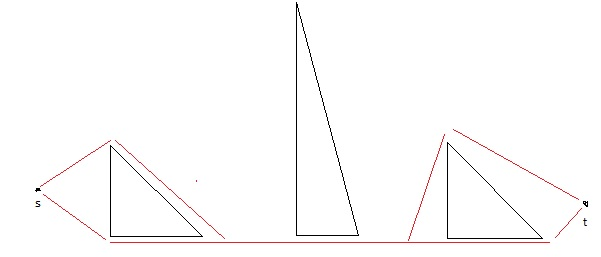
\includegraphics[height=3in]{shortestPaths_diagram.jpg}
\caption{Diagram of the shortest paths in the example above}
\end{figure}

There are $3n$ vertices total and each vertex is either in the shortest path or not in the shortest path, thus an upper bound on the total number of possible shortest paths is $2^{3n}$. \\
\\
To conclude:\\
Maximal Number of Shortest Paths Lower Bound: $2^{n/2}$\\
Maximal Number of Shortest Paths Upper Bound: $2^{3n}$ \\


\end{document}








